\section{Utilisation de symétries}

% \todoinline{Modification du titre et de l'ordre pour avoir segment / impropre et trigo / impropre et pas 1/x}
\begin{prop}{}{}
\[
\int_0^{\pi/4} \ln(1 + \tan x) \d x = \frac{\pi}{8} \ln(2).
\]
\end{prop}


\begin{exercice}
On pose $I = \int_0^{\pi/4} \ln(1+\tan x) \d x$.
\begin{questions}
\item Pour tout $x$ réel, exprimer $\cos x + \sin x$ en fonction de $\cos\mathopen{}\left(x - \frac{\pi}{4}\right)$.

\item En déduire la valeur de $I$.
\end{questions}
\end{exercice}

\begin{elemsolution}
L'intégrande est bien une fonction continue sur le segment $\interff{0}{\pi/4}$ donc l'intégrale est bien définie.
\begin{reponses}
\item En utilisant les formules d'addition,
\[
\cos x + \sin x = \sqrt{2} \cos\mathopen{}\left(x-\frac{\pi}{4}\right).
\]

\item On commence par substituer la fonction tangente pour faire apparaître des symétries :
\begin{align*}
\int_0^{\pi/4} \ln(1+\tan x) \d x &= \int_0^{\pi/4} \ln(1+\frac{\sin x}{\cos x}) \d x\\
 &= \int_0^{\pi/4} \ln(\sin x+\cos x) \d x - \int_0^{\pi/4} \ln(\cos x)\d x.
\end{align*}

On utilise ensuite la question précédente puis le changement de variable affine $u = \frac{\pi}{4} - x$ :
\begin{align*}
\int_0^{\pi/4} \ln(1+\tan x) \d x &= \int_0^{\pi/4} \ln\mathopen{}\big(\sqrt{2}\big) \d x + \int_0^{\pi/4} \ln(\cos x) \d x - \int_0^{\pi/4} \ln(\cos x) \d x\\
&= \frac{\pi}{8} \ln 2.
\end{align*}
\end{reponses}
\end{elemsolution}

\begin{marginfigure}[0cm]
    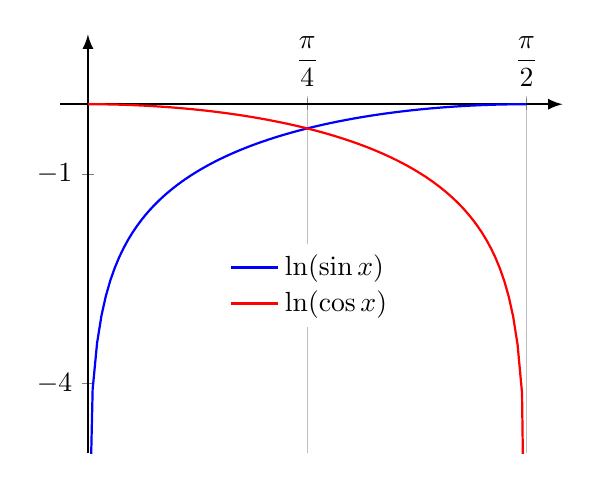
\begin{tikzpicture}
\begin{axis}[
    width=8cm,
    unit vector ratio*=1 0.5 1,
    xlabel={},
    ylabel={},
    xmin=-0.1, xmax=1.7,
    ymin=-5, ymax=1,
    xtick={0,0.7854,1.5708}, 
    xticklabel style={above=5pt},
    xticklabels={$0$,$\displaystyle \frac{\pi}{4}$,$\displaystyle \frac{\pi}{2}$},
    ytick={-1,-4},
    yticklabels={$-1$, $-4$},
    ticklabel style={fill=white},
    xmajorgrids,
    axis lines=middle,
    axis line style=thick,
    axis line style={-latex},
    samples=100,
    % legend pos=south center,
    legend style={
            at={(0.5,0.3)},
            anchor=south, 
            % at={(1.5708,0.5)},
            % anchor=north,
            legend cell align=left,
            draw=none % Unterdrücke Box
        },
]

\addplot[blue,thick, domain=0.001:1.5708] {ln(sin(deg(x)))};
\addplot[red,thick, domain=0.001:1.5708] {ln(cos(deg(x)))};
\legend{$\ln(\sin x)$, $\ln(\cos x)$}

\end{axis}
\end{tikzpicture}

\end{marginfigure}

% \todoinline{L'intégrale suivante semble s'appeler l'intégrale d'Euler - \url{https://fr.wikipedia.org/wiki/Table_d'intégrales}}

\begin{prop}[Intégrale d'\nom{Euler}]
\[
\int_0^{\pi/2} \ln(\sin x) \d x
= \int_0^{\pi/2} \ln(\cos x) \d x
= -\frac{\pi}{2} \ln(2).
\]
\end{prop}

\begin{exercice}[Intégrale d'\nom{Euler}]\label{exercice:integraleEuler}
\marginpar[0cm]{Source :  Oral - CCP-PSI-2016}
    Soient $I = \int_0^{\pi/2} \ln(\sin x) \d x$ et $J = \int_0^{\pi/2} \ln(\cos x) \d x$.
    \begin{questions}
        \item Montrer que $I$ et $J$ sont convergentes et que $I = J$.
        \item Calculer $I + J$ et en déduire $I$ et $J$.
    \end{questions}
\end{exercice}

% \todoinline{En mettre un peu plus sur la démo ? J'ai la version suivante à relire et changer les dt (CCP-PSI-2016) :}

\begin{elemsolution}
\begin{reponses}
\item La fonction $x \mapsto \ln(\sin x)$ est continue sur $\interof{0}{\pi/2}$. De plus, en $0$,
\[
\ln(\sin x) = \ln\mathopen{}\big(x + o(x)\big) = \ln(x) + \ln\mathopen{}\big(1 + o(1)\big) \sim_0 \ln x.
\]
Ainsi, d'après le théorème de comparaison des fonctions de signe constant, la fonction $x \mapsto \ln(\sin x)$ est intégrable en $0$.

Le changement de variable affine $\fonctionligne[\varphi]{u}{\frac{\pi}{2} - u}$ assure la convergence de $J$ ainsi que l'égalité $I = J$.

\item Comme ces intégrales sont bien définies, en utilisant la linéarité de l'intégrale et la symétrie dans la dernière égalité,
\begin{align*}
I + J &= \int_0^{\pi/2} \ln\mathopen{}\big( \sin(x) \cos(x) \big) \d x = \int_0^{\pi/2} \ln(\frac{\sin(2x)}{2}) \d x = \frac{1}{2} \int_0^\pi \ln(\sin x) \d x - \frac{\pi}{2} \ln(2) \\
&= I - \frac{\pi}{2} \ln(2).
\end{align*}
Ainsi, $I = J = -\frac{\pi}{2} \ln(2)$.
\end{reponses}
\end{elemsolution}
Voir le calcul de l'\hyperref[exercice:integralePoisson]{intégrale de \nom{Poisson}} pour une utilisation de l'intégrale d'\nom{Euler}.

\begin{prop}
\[
\int_0^{+\infty} \frac{x \ln(x)}{(1 + x^2)^2} \d x
= 0.
\]
\end{prop}

\begin{exercice}
On pose $I = \int_0^{+\infty} \frac{x \ln(x)}{(1 + x^2)^2} \d x$.
\begin{questions}
\item Montrer que l'intégrale $I$ est convergente.

\item En découpant l'intervalle $\interoo{0}{+\infty}$ en $\interfo{0}{1} \cup \interfo{1}{+\infty}$ et en effectuant un changement de variable, calculer~$I$.
\end{questions}
\end{exercice}

\begin{elemsolution}
\begin{reponses}
\item La fonction $f \colon x \mapsto \frac{x \ln(x)}{(1 + x^2)^2}$ est continue sur $\interoo{0}{+\infty}$.

Comme $f$ tend vers $0$ en $0$ par croissances comparées, on peut la prolonger par continuité en $0$ en posant $f(0) = 0$.

De plus, $\frac{x \ln(x)}{(1+x^2)^2} = o_{+\infty}\mathopen{}\left( \frac{1}{x^2} \right)$.

On en déduit que l'intégrale $\int_0^{+\infty} \frac{x \ln(x)}{(1 + x^2)^2} \d x$ converge.

\item D'après la relation de \textsc{Chasles},
\[
\int_0^{+\infty} \frac{x \ln(x)}{(1 + x^2)^2} \d x
= \int_0^1 \frac{x \ln(x)}{(1 + x^2)^2} \d x + \int_1^{+\infty} \frac{x \ln(x)}{(1 + x^2)^2} \d x.
\]

Dans la seconde intégrale, on effectue le changement de variable $\fonction[\varphi]{\interfo{1}{+\infty}}{\interof{0}{1}}{u}{\frac{1}{u}}$ qui est bien $\mathscr{C}^1$ et bijectif :
\begin{align*}
\int_0^{+\infty} \frac{x \ln(x)}{(1 + x^2)^2} \d x
&= \int_0^1 \frac{x \ln(x)}{(1 + x^2)^2} \d x + \int_0^1 \frac{\frac{1}{u} \ln \frac{1}{u}}{\big(1 + \frac{1}{u^2}\big)^2} \times \frac{1}{u^2} \d u\\
&= \int_0^1 \frac{x \ln(x)}{(1 + x^2)^2} \d x - \int_0^1 \frac{u \ln(u)}{(u^2 + 1)^2} \d u
= 0.
\end{align*}
\end{reponses}
\end{elemsolution}